\chapter{Statistical Analysis}
\label{chap:statistics}

\section{Introduction to Log Likelihood Fitting}
\label{sec:stat:likelihood}

\indent We check the consistency of data to predicted SM background and extract information on any potential signal using log likelihood fitting.  The basic premise behind log likelihood fitting is that the parameters most likely to describe the data is the one that maximizes the total likelihood defined in equation \ref{eqn:likelihood}.  \\

\begin{equation}
\label{eqn:likelihood}
{\mathcal{L}}(\vec{z}) = {\displaystyle\prod_{i=1}^{n}} P(x_i|\vec{z})
\end{equation}

\indent Where $x_i$ are data points and $\vec{z}$ are a list of parameters, and $P(x|\vec{z})$ is the fitted probability density function (PDF).  The PDF $P(x|\vec{z})$ have the probability of producing the a dataset $x_i$ when the likelihood is maximized. \\

\indent Maximizing the likelihood is equivalent to minimizing the negative log likelihood or NLL since logarithms are a monotonically increasing functions.  Therefore, we tend to minimize the NLL $M$ defined in equation \ref{eqn:NLL} \\

\begin{equation}
\label{eqn:NLL}
M(\vec{z})=-\ln(({\mathcal{L(\vec{z})}}) = -{\displaystyle\sum_{i=1}^{n}} \ln( P(x_i|\vec{z}) )
\end{equation}

\indent In collider physics we do not know the total number of $n$ events a priori.  Instead, we have an expected value of events proportional to the cross-section times luminosity.  This means the actual number of measured events should vary according to a poisson distribution.  We include this uncertainty in the number of final observed events by multiplying a poisson distribution with expected rate $\lambda$ to the likelihood in equation \ref{eqn:likelihood} resulting in equation \ref{eqn:ExtLikelihood}.  \\

\begin{equation}
\label{eqn:ExtLikelihood}
{\mathcal{L}}(\vec{z}) = \{ \frac{\exp^{-\lambda}{\lambda}^n}{n!} \}  {\displaystyle\prod_{i=1}^{n}} P(x_i|\vec{z})
\end{equation}

\indent Finally, for this particular analysis we perform a binned fit to the $\RISR$ distribution in the signal region instead of an event by event shape fit.  Therefore our fitted PDF $(x_i|\vec{z})$ is not a full continuous function but a series of expected values in discrete bins.  Therefore $P(x|\vec{z})$ can be written as equation \ref{eqn:binnedPDF}. \\

\begin{equation}
\label{eqn:binnedPDF}
P_{b_i} = P(x_i|\vec{z}) = \int^{b_i}_{b_{i-1}} f(x|\vec{z})
\end{equation}

Where $f(x|\vec{z})$ is the continuous PDF, $b_i$ and $b_{i-1} $ are the bin edges for the ith bin. Assuming a poisson distribution of events in each bin, the extended likelihood and NLL becomes equation \ref{eqn:binnedlikelihood} and \ref{eqn:binnedNLL}.

\begin{equation}
\label{eqn:binnedlikelihood}
{\mathcal{L}}(N^{data}_{b_i}|\vec{z}) = {\displaystyle\prod_{k=1}^{n_{bins}} \frac{({\lambda}P_{b_i})^{N^{data}_{b_i}}e^{-{\lambda}P_{b_i}}}{N^{data}_{b_i}!}}
\end{equation}
\begin{equation}
\label{eqn:binnedNLL}
M(\vec{z})=-\ln(({\mathcal{L(\vec{z})}}) = -{\displaystyle\sum_{i=1}^{n_bins}} ( N^{data}_{b_i} \ln( {\lambda}P_{b_i} ) - {\lambda}P_{b_i} - \ln{N^{data}_{b_i}!}
\end{equation}

\indent Where $N^{data}_{b_i}$ is the number of data in the ith bin, $\lambda$ is the expected rate in the region, $P_{b_i}$ is the probability of an event being in the ith bin if it is in the signal region and $\vec{z}$ is the fitted parameters such as signal cross-section etc.   Both $\lambda$ and $P_{b_i}$ can depend on the fitted parameters $\vec{z}$ because the total amount and shape of background and signal can change with the fitted parameters. \\

\indent A mathematically equivalent interpretation is that ${\lambda}P_{b_i}$ is simply the expected number of events in a particular bin.  In this case, equation \ref{eqn:binnedlikelihood} and \ref{eqn:binnedNLL} become \ref{eqn:binnedlikelihood2} and \ref{eqn:binnedNLL2} where $N^{MC}_{b_i}$ is the expected number of events from simulation. \\

\begin{equation}
\label{eqn:binnedlikelihood2}
{\mathcal{L}}(N^{data}_{b_i}|\vec{z}) = {\displaystyle\prod_{k=1}^{n_{bins}} \frac{(N^{MC}_{b_i})^{N^{data}_{b_i}}e^{-N^{MC}_{b_i}}}{N^{data}_{b_i}!}}
\end{equation}

\begin{equation}
\label{eqn:binnedNLL2}
M(\vec{z})=-\ln(({\mathcal{L(\vec{z})}}) = -{\displaystyle\sum_{i=1}^{n_bins}} ( N^{data}_{b_i} \ln( N^{MC}_{b_i} ) - N^{MC}_{b_i} - \ln{N^{data}_{b_i}!}
\end{equation}

\indent Simultaneous fits to multiple regions is performed by simultaneously maximizing the total negative log likelihood of all fitted regions.  The total negative log likelihood is simply a sum of the individual likelihood of each region.  \\

\section{Overview of Fitting to Control Regions and Signal Regions}
\label{sec:stat:Bkg}

\indent We hope to both predict the number of expected background events and extract the amount of signal present by performing log likelihood fits to the control regions and signal region in our analysis.  

\indent We normalize backgrounds to data in control regions dominated by background but are kinematically similar to the signal region.  The background normalization is allowed to float and the fit will extract the total amount of background that best describe the data in all the different control regions. All backgrounds that form a statistically significant contribution to the total background in SR has a corresponding CR.  The background estimation techniques and definitions of these CRs are given in chapter \ref{chap:backgrounds}.  \\

\indent The amount of MC background in both the CR and SR will fluctuate with experimental and theoretical systematics for the fit.  However after the fit the total amount of background will be normalized to the CR.  If the raw MC yield for background fluctuate down with a given systematic then the normalization scale factor in the CR will increase.  If the raw MC background yield in SR also decreases by the same amount, then the increased normalization scale factor will compensate for this and bring fitted background yield in SR remains unchanged.  In this way, the control region help cancel systematic variations by directly measuring the amount of background in from data instead of relying on MC predictions.  \\

\indent The more kinematically similar the definition of the CR to the SR, the better the cancelation.  Any extrapolation between CR and SR must only be across well modeled variables.  Otherwise large systematic uncertainties will arise due to extrapolation cross poorly modeled parts of the simulation or worse the background prediction maybe wrong.  \\

\indent We can also check the result of our background predictions without unblinding the signal region in validation regions.  Validation regions receive the normalization scale factors to background from the fit to the control region but do not participate in the fit.   The VRs are designed to be kinematically similar to the SRs while keeping signal contaminations low.  In this way, the VRs serves as a mid-point to check the extrapolation between CR and SR.  \\

\indent The relationship between CR, SR and VR is graphically depicted in figure \ref{fig:CR_VR_SR_stat}. \\

\begin{figure}[h!]
  \centering
	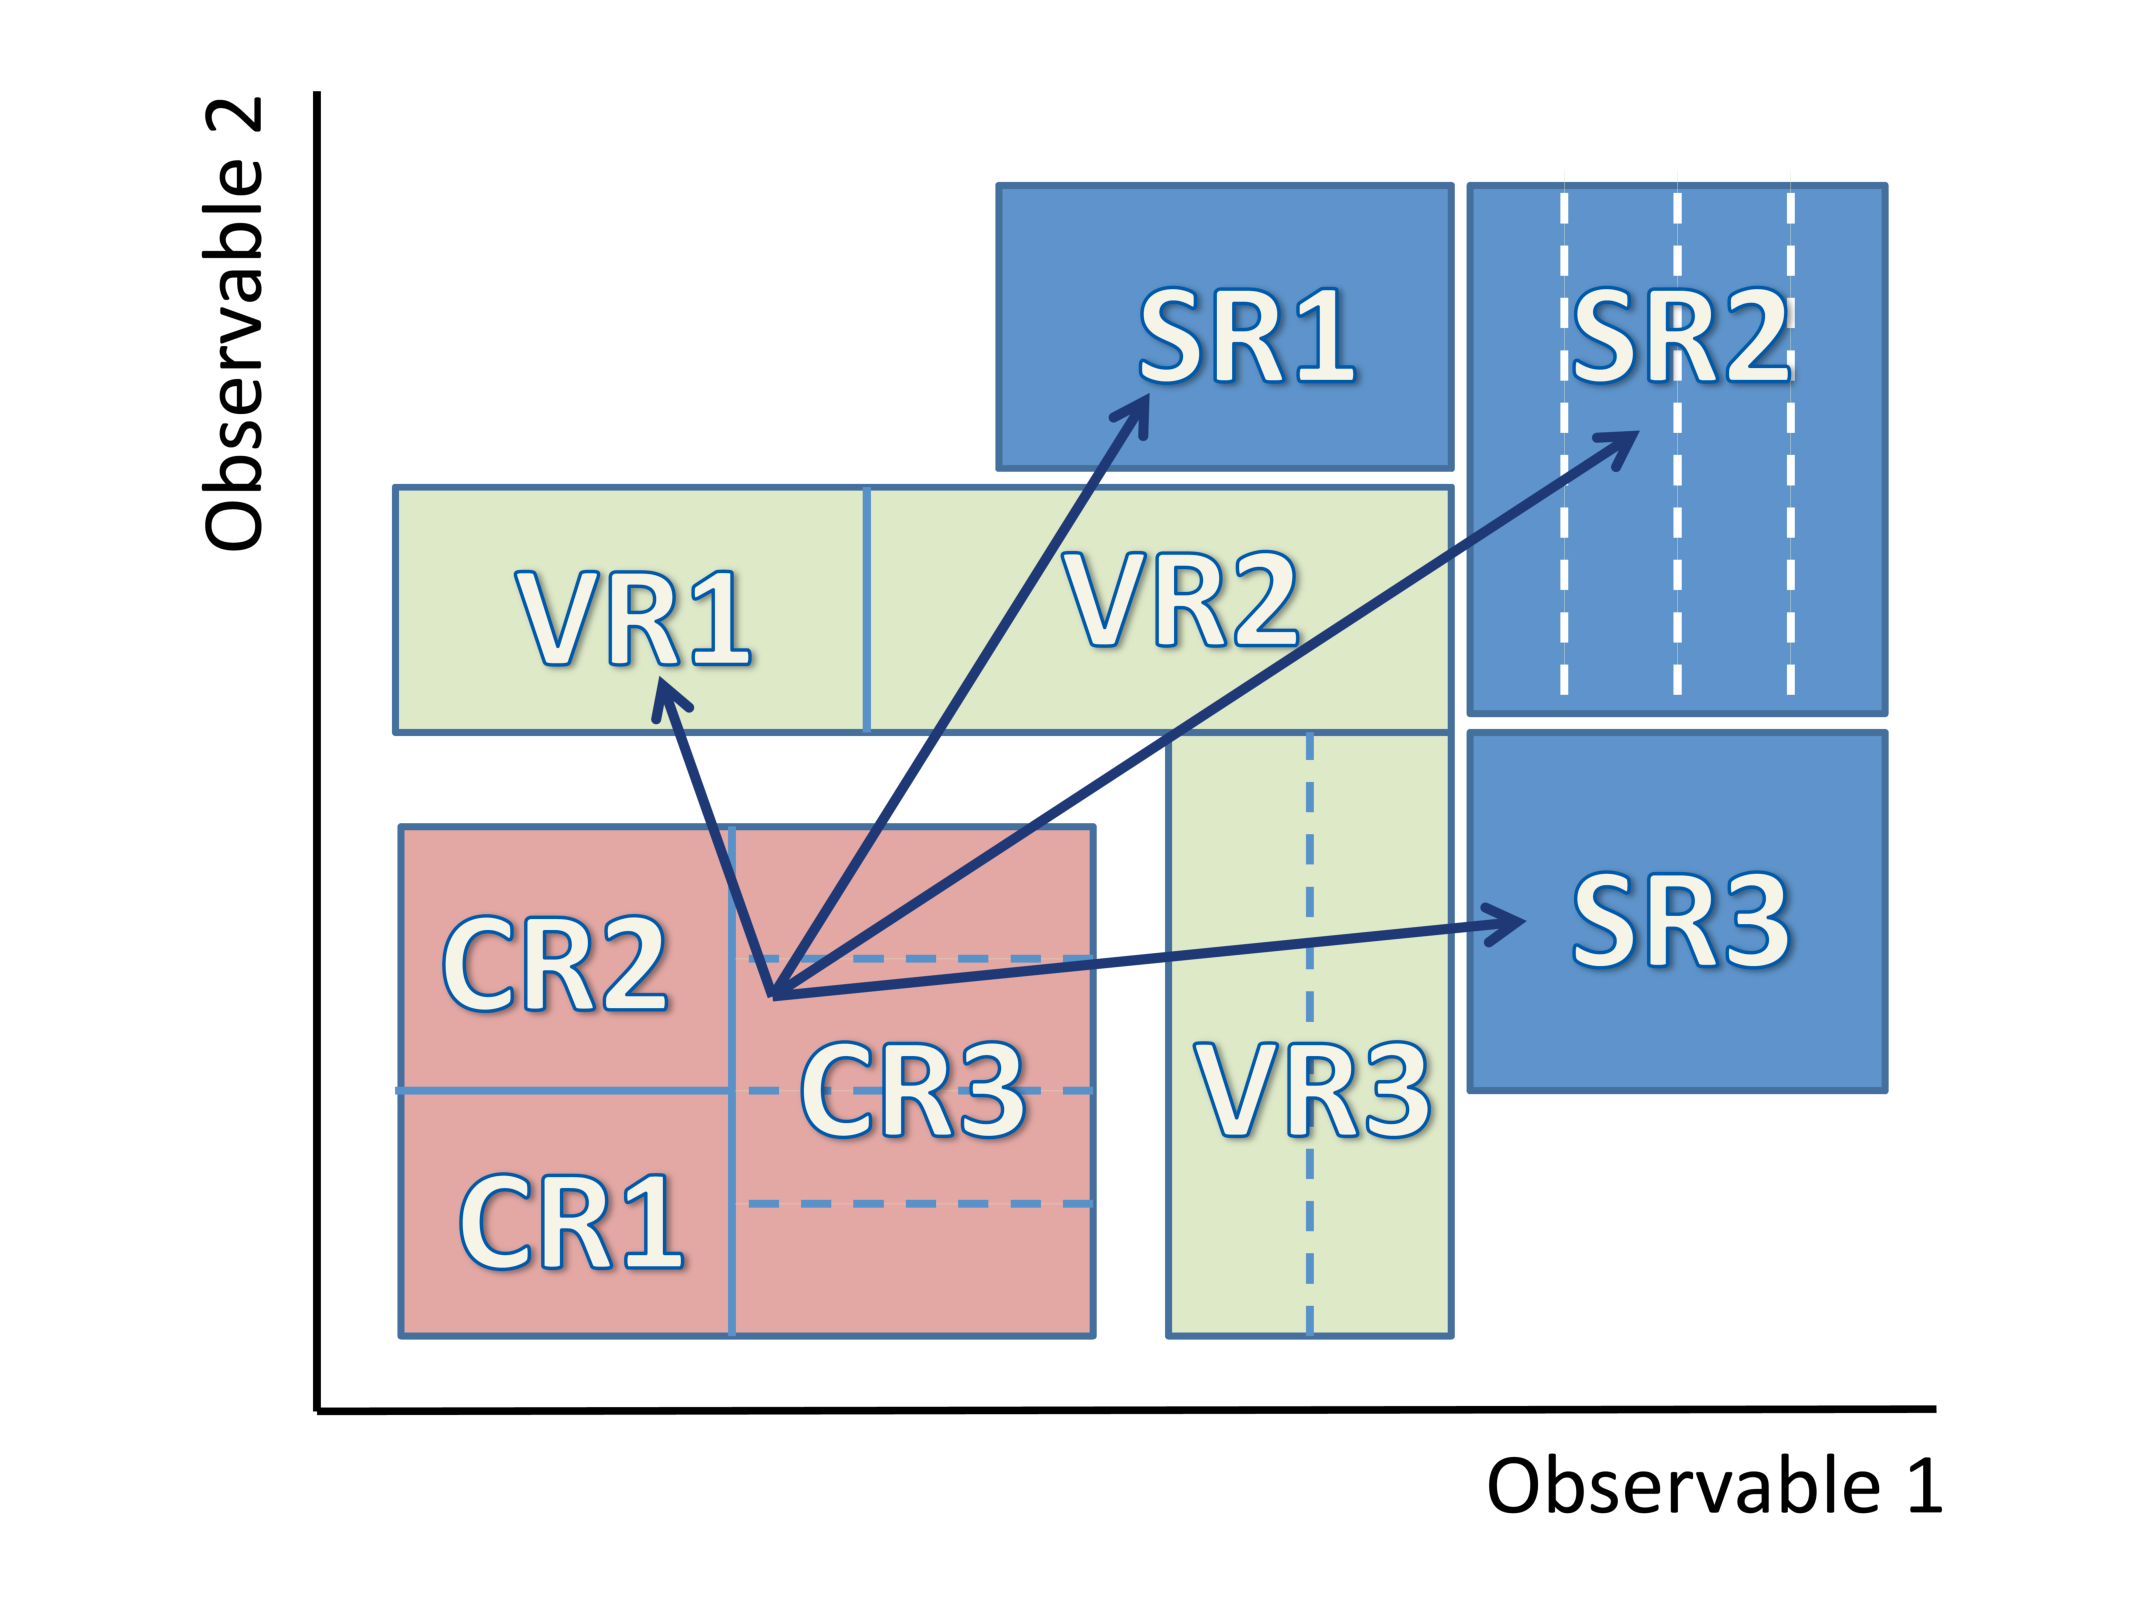
\includegraphics[width=0.65\textwidth]{./figures/statistics/CR_VR_SR.pdf}
\caption{\label{fig:CR_VR_SR_stat}{Basic diagram of data driven background estimation techniques.  We define control regions (CR) that is dominated by background and have little signal.  We can estimate the amount of background we expect in the signal region (SR) by measuring the amount of background in the CR and extrapolating to the SR using MC predictions. }}
\end{figure}

\indent In an excess were to exist in the SR, a simultaneous fit to all CR and SR is performed for to calculate the statistical significance of any potential excess in the case of discovery.   If no excess were found, then a simultaneous fit to all CR and SR is also performed quantify the maximum amount of signal cross-section that can be excluded.  \\

\indent The background normalization and systematic uncertainty is also extracted through these simultaneous fit to control and signal regions. \\

\indent However, the CRs have much higher statistics then the SR.  Therefore, the background rate is mainly constrained by the CR and the SR mainly constrain the amount of signal.  Therefore we can quantify the amount of background and the systematic uncertainty that we would expect in the signal region by perform a background only fit where only CRs are fitted.  In this case, the SR behaves like another VR and is not fitted.  \\

\indent These three type of fits, the background only fit, the discovery fit and the exclusion fit are covered in more detail in sections \ref{sec:stat:bkgonly} to \ref{sec:stat:limit}. The parameterization of systematics as constrained nuisance parameters is covered in section \ref{sec:stat:sys}. \\

\indent We use the software package \HistFitter (version {\tt HistFitter-00-00-53} ) to perform the statistical analysis.\cite{HistFitter}  \HistFitter provide many tools tools to easily manage and integrate multiple CR, SR backgrounds, and systematics.  \HistFitter is built upon other statistical analysis software including \RooFit.\cite{RooFit} At its core \HistFitter is still performing log likelihood fitting based on the principle introduced in section \ref{sec:stat:likelihood} but the software makes bookkeeping of the different CR, SRs and fits much more streamlined. \\

\section{Parameterization of Systematics as Gaussian Constraints}
\label{sec:stat:sys}

\indent Systematics uncertainties are parameterized as fitted parameters called nuisance parameters.  The nuisance parameter, defined as $\alpha$, is constrained to a particular value by a constraint function $C(\alpha)$.   The fitted PDF $P(x|\vec{z},\alpha)$ can depend on a number of unconstrained fitted parameter $\vec{z}$ and the constrained $\alpha$.  The constraint function $C(\alpha)$ is multiplied to the likelihood as shown in equation \ref{eqn:stat:sys} and contributes to the total likelihood.  

\begin{equation}
\label{eqn:stat:sys}
{\mathcal{L}}(\vec{z},\alpha) = {\displaystyle\prod_{i=1}^{n}} P(x_i|\vec{z},\alpha) C(\alpha)
\end{equation}

\indent Now the value of $\alpha$ corresponding to the maximum likelihood ${\mathcal{L}}(\vec{z},\alpha)$ may not be the same as value where $C(\alpha)$ is maximized.  Depending on the data points $x_i$, the component of the likelihood from ${\displaystyle\prod_{i=1}^{n}} P(x_i|\vec{z},\alpha)$ maybe bigger even if $C(\alpha)$ is not at its maximum. \\

\indent We pay a penalty on the total likelihood if the nuisance parameter $\alpha$ deviates from the value with maximum $C(\alpha)$.  The fit finds the optimal point between changing the $\alpha$ so that the PDF best describes the data and the cost from the constraint function on $\alpha$. \\

\indent We use Gaussians as the constraint function for all systematics.  The nominal value corresponds to $\alpha = 0$ and the plus and minus 1 sigma deviation corresponds to $\alpha = \pm1$.  \\

\indent Two types of systematics exist normalization and shape for our analysis.  Normalizations systematics are only applied to the total normalization of the background and signal in the SR.  For normalization background we determine how much the backgrounds and signal will fluctuate with the $\pm1$ sigma variation in systematic in each of our CRs and SR.  \\

\indent Shape systematics on the other allow different bins in $\RISR$ in the SR to fluctuate at different rates differently.  For example a shape systematic with the $\alpha$ value of 0.1 and have a 10 percent increase in background in bin 1 but a 15 percent increase in background in bin 2.  The fluctuation in each bin is determined independently.  \\

\section{Background Only Fit and Background Estimation}
\label{sec:stat:bkgonly}

\indent For the background only fit, the CRs are simultaneously fitted but the SR is not fitted.  The backgrounds in the SR are normalized to the background normalization scale factors derived from the fit to the CRs.  No signal sample is included in the fit and potential signal contamination in the CR is ignored.  The background only fit is performed to estimate the background systematic uncertainties and the amount of expected background in the signal region in the absence of an signal.  \\

\indent The background only fit has the advantage of being able to quantify the expected amount of background and systematic uncertainties on background while the SR is blinded.  \\

\indent The background normalizations predicted in the background only fit may differ from the discovery and exclusion fits because the SR is simultaneously fitted in those fits. This difference should be small as long as the CRs are well designed and have much higher constraining power on the amount of background then the SR.  The CRs that have high purity in a single background and high statistics will have much stronger constraining power on the amount of background then the lower statistics SR.  \\

\section{Exclusion Fit and Exclusion Limit Calculation}
\label{sec:stat:limit}

\indent The exclusion fit is performed as a simultaneous fit to all CRs and SR.  The signal sample is included in both CR and SR and normalized to a signal strength parameter.  The signal strength parameter can be varied but is constrained to be non-negative.  The five bins in $\RISR$ is simultaneously fitted in the SR for exclusion.  \\

\indent The best fit signal strength is found when the negative log likelihood (NLL) is at a minimum after fitting to data.  As the signal strength deviates from the best fit value, the NLL increases and we are more confident that the signal strength is not supported by data.  The NLL's variation and the statistical significance should be related to one another by a parabola if the statistics in SR is high enough.  The signal strength corresponding to when the NLL is $1$ above the minimum NLL corresponds to the 1 sigma confidence interval on signal strength.  The signal strength corresponding to when the NLL is $4$ above the minimum NLL corresponds to the 2 sigma confidence interval on signal strength and so on. \\

\indent In other words, we use the difference in NLL as our test statistic and the relationship between the test statistic and statistical significance approaches the asymptotic case of of a parabola at high statistics. \\

\indent In this way we can find the 95 percent confidence interval on the signal cross-section.  If the high end of the 95 percent confidence interval on signal cross-section is less then the production cross-section of a particular signal model then that signal model has been excluded to at least 95 confidence.  \\

\indent Alternatively we can calculate the NLL corresponding to the nominal signal strength of each signal model and compare it with the fitted minimum NLL.  The difference in the two NLLs can be converted into the statistical significance using the parabolic relationship between the two.  The statistical significance of the nominal signal strength for a particular model is the exclusion p-value for the model.  If the exclusion p-value is below 5 percent then the signal model has been excluded to 95 confidence. \\

\indent We calculate the exclusion p-value corresponding to a grid of signal models each with a different stop and neutralino mass.  The p-values are plotted in a 2D graph with the stop mass along the x-axis and the neutralino mass along the y-axis.  These p-values are then interpolated over to form a 2D contour plot.  The contour corresponding to the 95 percent exclusion limit is then draw. \\

\section{Discovery Fit and Discovery Significance Calculation}
\label{sec:stat:discovery}

\indent The discovery fit is also performed as a simultaneous fit to all CRs and SR.  The signal sample is included only in the SR but not to the CR in the fit.  This choice of excluding the signal sample from the CR gives a more conservative estimate of the discovery significance.  If a signal is present in nature, the signal contamination in the CR would still exist in data.  We essentially over-estimate the amount of background by counting any potential signal contamination in the CR as background.  Again, a well designed CR has little signal contamination so the difference between this approach and exclusion fit should be small.  Our signal contamination is less then 15 percent for all signal samples that we are sensitive to but have not been excluded by previous 8 TeV ATLAS analysis.  The signal contamination is less then 10 percent for all stop masses above 300 GeV.  \\  

\indent We do not statically combine the 5 $\RISR$ bins for the discovery fit.  Instead a single $\RISR$ bin is fitted at a time and the bin with the best significance is used as the discovery significance for the signal model.  Again this is a conservative approach and gives us worse discovery significances but it makes the analysis less sensitive to shape uncertainties in signal.  \\

\indent We also use the difference in NLL as our test static for our discovery fit.  The signal strength and background normalization that best fit the data is found at the minimum NLL.  Then we calculate the NLL with a signal strength of zero.  The difference between the NLL with a signal strength of zero and the best fit NLL is our test statistic.  The relationship between the test statistic is given by a parabola in the asymptotic high statistics case. We assume we are in the asymptotic case and derive the statistic significance of the zero signal strength fit.  \\

\indent The statistical significance of the zero signal strength fit represent the amount of disagreement between data and the no signal case.  In other words, the statistical significance of the zero signal strength fit is the p-value of the no signal hypothesis test.  This p-value is the discovery significance for the analysis.  If the discovery significance is above 5 sigma then discovery can be claimed.\\

